\documentclass[11pt]{article}

\usepackage[a4paper,left=2.5cm,right=2.5cm,top=3.5cm,bottom=3.5cm]{geometry}
\usepackage[utf8]{inputenc}
\usepackage[T1]{fontenc}
\usepackage[english]{babel}
\usepackage{graphicx}
\usepackage{amsmath,amssymb,amsthm,amsopn}
\usepackage{mathrsfs}
\usepackage{graphicx}
\usepackage{array}
\usepackage{makecell}
\usepackage{bm}
\usepackage{hyperref}
\usepackage[shortlabels]{enumitem}
\hypersetup{
    colorlinks=true,
    linkcolor=blue,
    citecolor=red,
}
\usepackage{diagbox}

\usepackage{algorithm}
\usepackage{algpseudocode}

\renewcommand{\algorithmicrequire}{\textbf{Input:}}
\renewcommand{\algorithmicensure}{\textbf{Output:}}

%\usepackage[top=1cm,bottom=1cm]{geometry}
%\usepackage{listings}
%\usepackage{xcolor}

\usepackage{tikz}
\usetikzlibrary{arrows}

% Tikz style

\tikzset{round/.style={circle, draw=black, very thick, scale = 0.7}}
\tikzset{arrow/.style={->, >=latex}}
\tikzset{dashed-arrow/.style={->, >=latex, dashed}}

\newtheoremstyle{break}%
{}{}%
{\itshape}{}%
{\bfseries}{}%  % Note that final punctuation is omitted.
{\newline}{}

\newtheoremstyle{sc}%
{}{}%
{}{}%
{\scshape}{}%  % Note that final punctuation is omitted.
{\newline}{}

\theoremstyle{break}
\newtheorem{thm}{Theorem}[section]
\newtheorem{lm}[thm]{Lemma}
\newtheorem{prop}[thm]{Proposition}
\newtheorem{cor}[thm]{Corollary}

\theoremstyle{sc}
\newtheorem{exo}{Exercice}

\theoremstyle{definition}
\newtheorem{defi}[thm]{Definition}
\newtheorem{ex}[thm]{Example}

\theoremstyle{remark}
\newtheorem{rem}[thm]{Remark}

% Math Operators

\DeclareMathOperator{\Card}{Card}
\DeclareMathOperator{\Gal}{Gal}
\DeclareMathOperator{\Id}{Id}
\DeclareMathOperator{\Img}{Im}
\DeclareMathOperator{\Ker}{Ker}
\DeclareMathOperator{\Minpoly}{Minpoly}
\DeclareMathOperator{\Mod}{mod}
\DeclareMathOperator{\Ord}{Ord}
\DeclareMathOperator{\ppcm}{ppcm}
\DeclareMathOperator{\tr}{Tr}
\DeclareMathOperator{\Vect}{Vect}
\DeclareMathOperator{\Span}{Span}
\DeclareMathOperator{\rank}{rank}
\DeclareMathOperator{\ev}{ev}

% Shortcuts

\newcommand{\dE}{\partial(E)}
\newcommand{\dF}{\partial(F)}
\newcommand{\dG}{\partial(G)}
\newcommand{\diff}{\mathop{}\!\mathrm{d}}
\newcommand{\eg}{\emph{e.g. }}
\newcommand{\emb}{\hookrightarrow}
\newcommand{\embed}[2]{\phi_{#1\hookrightarrow#2}}
\newcommand{\ent}[2]{[\![#1,#2]\!]}
\newcommand{\ie}{\emph{i.e. }}
\newcommand{\ps}[2]{\left\langle#1,#2\right\rangle}
\newcommand{\eqdef}{\overset{\text{def}}{=}}
\newcommand{\f}{f}%{\mathfrak{f}}
\newcommand{\bff}{\mathbf{f}}
\newcommand{\E}{\mathcal{E}}
\newcommand{\A}{\mathcal{A}}
\newcommand{\B}{\mathcal{B}}
\newcommand{\R}{\mathcal{R}}
\newcommand{\bfa}{\mathbf{a}}
\newcommand{\bfb}{\mathbf{b}}
\newcommand{\D}{\mathcal{D}}
\newcommand{\Pcal}{\mathcal{P}}
\newcommand{\musym}{\mu^{\textrm{sym}}}
\newcommand{\mutri}{\mu^{\textrm{tri}}}
\newcommand{\muhyp}{\mu^{\textrm{hyp}}}
\newcommand{\musymG}[1][G]{\mu^{\textrm{sym},#1}}
\newcommand{\mutriG}[1][G]{\mu^{\textrm{tri},#1}}
\newcommand{\muhypG}[1][G]{\mu^{\textrm{hyp},#1}}
\newcommand{\hmusym}{\hat\mu^{\textrm{sym}}}
\newcommand{\hmutri}{\hat\mu^{\textrm{tri}}}
\newcommand{\hmuhyp}{\hat\mu^{\textrm{hyp}}}
\newcommand{\hmusymG}[1][G]{\hat\mu^{\textrm{sym},#1}}
\newcommand{\hmutriG}[1][G]{\hat\mu^{\textrm{tri},#1}}
\newcommand{\hmuhypG}[1][G]{\hat\mu^{\textrm{hyp},#1}}
\newcommand{\Msym}{M^{\textrm{sym}}}
\newcommand{\Mtri}{M^{\textrm{tri}}}
\newcommand{\Mhyp}{M^{\textrm{hyp}}}
\newcommand{\hMsym}{\hat{M}^{\textrm{sym}}}
\newcommand{\hMtri}{\hat{M}^{\textrm{tri}}}
\newcommand{\hMhyp}{\hat{M}^{\textrm{hyp}}}
\newcommand{\tri}[2]{\mu_{#1}^{\text{tri}}(#2)}
\newcommand{\sym}[2]{\mu_{#1}^{m_3}(#2)}
\newcommand{\K}{\mathbf{k}}


% opening
\title{Trisymmetric multiplication formulae in finite fields}
\author{}



\begin{document}

\maketitle

\begin{abstract}
  To be written.
\end{abstract}

%\tableofcontents
%\clearpage

\section{Introduction}
\label{sec:intro}

%\paragraph{Bilinear complexity.}
Given an algorithm that computes a polynomial map over a field $\K$
(or a family of such polynomial maps, with entries of length going to infinity),
one is
usually interested in the (asymptotic) cost of the algorithm. In order to
understand this cost, one studies the \emph{complexity} of the algorithm, \ie
the number of operations needed by the algorithm. We can for example count the number
of bit operations, or the number of algebraic operations $(+, \times)$ in $\K$. The latter is called the \emph{algebraic complexity}
and in this model it is supposed that all algebraic operations have the same cost.
Nevertheless, multiplication of two variable quantities in $\K$ is arguably more expensive than
addition, or than multiplication of a variable by a fixed constant. In the context of the computation of
bilinear maps, extensive work has been done to reduce the number of
two-variable multiplications involved. Notable examples are Karatsuba's
algorithm~\cite{Karatsuba63} and
Strassen's algorithm~\cite{Strassen69}. Karatsuba's algorithm is
based on the fact that the bilinear map associated to the product of two
polynomials of degree $1$
\[
  A = a_1 X + a_0\text{ and }B = b_1 X + b_0
\]
can be computed with three products $a_0b_0, (a_0+a_1)(b_0+b_1), a_1b_1$ instead
of the four classic ones $a_0b_0, a_0b_1, a_1b_0, a_1b_1$. Strassen's algorithm
exploits a similar idea in the case of $2\times2$ matrices: only $7$ products
are used instead of $8$ in order to compute a matrix product. Both these
algorithms have very practical consequences. The \emph{bilinear complexity}
$\mu(\Phi)$ of a bilinear map $\Phi$ over $\K$ represents the minimum number of two-variable
multiplications in a formula that computes $\Phi$, discarding the cost of other
operations such as addition or multiplication by a constant.
%The bilinear complexity is defined as the minimal number $n$ such that there exist
%linear forms $(\varphi_i)_{1\leq i \leq n}$, $(\psi_i)_{1\leq i \leq n}$ in
%$\A^\vee$, where $\A^\vee$ is the dual of $\A$, and
%elements $(a_i)_{1\leq i \leq n}$ in $\A$ such that
%\begin{equation}
%  \forall x, y\in\A,\,xy = \sum_{i=1}^{n}\varphi_i(x)\psi_i(y)a_i.
%  \label{eq:no-sym}
%\end{equation}
%Equivalently, it can be defined as the rank of the tensor in
%\[
%  \A^\vee \otimes \A^\vee\otimes \A
%\]
%corresponding to the multiplication map in $\A$.
In particular when $\A$ is a finite dimensional algebra over $\K$,
we define the bilinear complexity of $\A$ as $\mu(\A/\K)=\mu(m_{\A})$
where $m_{\A}:\A\times\A\to\A$ is the multiplication map in $\A$ seen
as a $\K$-bilinear map. 

Let $\K^{2\times2}$ be the algebra
of $2\times2$ matrices over $\K$. We know thanks to Strassen's algorithm that 
\[
  \mu(\K^{2\times 2}/\K) \leq 7.
\]
In fact, this is optimal, so we have exactly $\mu(\K^{2\times2}/\K)=7$. In
general, it seems to be hard to find the bilinear complexity of a given algebra,
for example the bilinear complexity of $\K^{3\times3}$ is not known.
In the litterature, work has been done both to algorithmically find the bilinear complexity of
small algebras~\cite{BDEZ12, Covanov19} and to understand how the bilinear
complexity asymptotically grows~\cite{CC88, BCPRRR19}. Chudnovsky and Chudnovsky
proved in 1988 that the bilinear complexity of an extension field
$\mathbb{F}_{q^k}/\mathbb{F}_{q}$ is linear in the degree $k$ of the
extension, using an evaluation-interpolation method on curves.
As the main contribution of this article, we
investigate both questions for \emph{trisymmetric} bilinear complexity.

When a bilinear map admits certain invariance properties, it can be interesting,
both for theoretical and for practical reasons,
to find formulae for it that exhibit these same invariances.
For symmetric bilinear maps, and in particular for commutative algebras, this leads to the notion of symmetric bilinear complexity.
A further refinement, the trisymmetric bilinear complexity of $\mathbb{F}_{q^k}$ over $\mathbb{F}_{q}$, was first introduced in \cite{SL84}, and rediscovered independently in \cite[App.~A]{Randriam15}.

In Section~\ref{sec:symtrisym} we recall the definition of symmetric and trisymmetric formulae, and discuss further generalizations. In Section~\ref{sec:algos} we
describe algorithms to compute trisymmetric decompositions in small dimension.
Finally, in
Section~\ref{sec:asymptotic}, we prove (among other generalizations) that for all $q\geq2$, the trisymmetric bilinear
complexity of an extension of $\mathbb{F}_q$ is again linear in the degree.
All these results solve a certain number of open problems 5.2 from \cite{BCPRRR19}.

\section{Multiplication formulae with symmetries}
\label{sec:symtrisym}

Although we are mainly interested in bilinear multiplication formulae,
the notions we will consider naturally involve higher multilinear maps.

\paragraph{Multilinear complexity.}
Let $\Phi:V_1\times\cdots\times V_s\to W$
be a $s$-multilinear map between finite dimensional vector spaces over $\K$.
A \emph{multilinear algorithm}, or \emph{multilinear decomposition}, or \emph{multilinear formula} of length $n$ for $\Phi$ is a collection linear
forms $(\phi_i^{(j)})_{\substack{1\leq i \leq n\\1\leq j\leq s}}$,
where $\phi_i^{(j)}$ is in $V_j^\vee$, the dual vector space of $V_j$,
and elements $(w_i)_{1\leq i \leq n}$ in $W$, 
such that for all $v_1,\dots,v_s$ we have
\[
  \Phi(v_1,\dots,v_s)=\sum_{i=1}^{n}\varphi_i^{(1)}(v_1)\cdots\varphi_i^{(s)}(v_s)w_i.
\]
The \emph{multilinear complexity} $\mu(\Phi)$ is then defined as the smallest
length $n$ of such a decomposition.
Equivalently, it is the rank of the tensor in
$V_1^\vee \otimes\dots\otimes V_s^\vee\otimes W$
corresponding to $\Phi$.

\paragraph{Symmetric multilinear complexity.}
When $V_1=\cdots=V_s=V$ and $\Phi$ is a \emph{symmetric} multilinear map, it is
natural to search for \emph{symmetric multilinear decompositions}, \ie formulae of the form
\begin{equation*}
  \Phi(v_1,\dots,v_s)=\sum_{i=1}^{n}\varphi_i(v_1)\cdots\varphi_i(v_s)w_i
%  \label{eq:sym}
\end{equation*}
with $\varphi_i^{(1)}=\dots=\varphi_i^{(s)}=\varphi_i\in V^\vee$ for all $i$.
It is more space-efficient, since symmetric formulae admit a shorter description.
On an algorithmic point of view, it should also be simpler to find symmetric formulae,
because the search space is smaller. 
We define $\musym(\Phi)$,
the \emph{symmetric multilinear complexity} of $\Phi$,
as the minimal length $n$ of such a symmetric decomposition, if it exists
(otherwise we set $\musym(\Phi)=\infty$).

In the case $s=2$, a symmetric bilinear map always admits a symmetric decomposition.
However, when $s\geq3$ and $\K=\mathbb{F}_q$ is a finite field, this can fail.
When $s=3$ and $q>2$, it is shown in \cite[Lemma~7]{SL84} that a symmetric trilinear map $\Phi$ over $\mathbb{F}_q$ always admits a symmetric algorithm,
while in the remaining case $s=3$ and $q=2$, as observed by Cascudo,
a necessary condition is that $\Phi$ should satisfy $\Phi(x,x,y)=\Phi(x,y,y)$
for all entries $x,y$.
These results were then combined and generalized into the following necessary and sufficient criterion:
\begin{thm}[{\cite[Thm.~A.7]{Randriam15}}]\label{criterion}
Let $\Phi:V^s\to W$ be a $s$-multilinear map between finite dimensional vector spaces over $\mathbb{F}_q$.
Then $\Phi$ admits a symmetric decomposition if and only if $\Phi$ is \emph{Frobenius-symmetric},
\ie if and only if it is symmetric and one of the following two conditions holds:
\begin{itemize}
\item $s\leq q$
\item $s\geq q+1$ and for all $u,v,z_1,\dots,z_{s-q-1}$ in $V$,
\[
\Phi(\underset{\textrm{$q$ times}}{\underbrace{u,\dots,u}},v,z_1,\dots,z_{s-q-1})=\Phi(u,\underset{\textrm{$q$ times}}{\underbrace{v,\dots,v}},z_1,\dots,z_{s-q-1}).
\]
\end{itemize}
\end{thm}
Observe that this criterion involves the \emph{cardinality} of the field, not its characteristic.

\paragraph{Trisymmetric and hypersymmetric complexity.}
Now suppose furthermore that $V=W$, and that this space is equipped with a
non-degenerate symmetric bilinear form, written as a scalar product
\[
\begin{array}{ccc}
V\times V &\to&\K\\
(v,w)&\mapsto&\ps{v}{w}.
\end{array}
\]
This allows to identify $V$ and $V^\vee$, \ie any linear form $\phi\in V^\vee$
is of the form $\phi(x)=\ps{a}{x}$ for a uniquely determined $a\in V$.
As a consequence, a symmetric decomposition for $\Phi:V^s\to V$ can also be described
as the data of elements $(a_i)_{1\leq i\leq n}$ and $(b_i)_{1\leq i\leq n}$ in $V$
such that for all $v_1,\dots,v_s$ in $V$,
we have $\Phi(v_1,\dots,v_s)=\sum_{i=1}^{n}\ps{a_i}{v_1}\cdots\ps{a_i}{v_s}b_i$.
In order to have an even more compact description, one could ask for $b_i$ to be proportional to $a_i$, leading to the following:
\begin{defi}
Let $V$ be a finite dimensional $\K$-vector space equipped with a scalar product,
and $\Phi:V^s\to V$ a symmetric $s$-multilinear map.
Then a \emph{hypersymmetric} formula for $\Phi$ is the data of
elements $(a_i)_{1\leq i\leq n}$ in $V$ and scalars $(\lambda_i)_{1\leq i\leq n}$ in $\K$ such that, for all $v_1,\dots,v_s\in V$,
\[
\Phi(v_1,\dots,v_s)=\sum_{i=1}^{n}\lambda_i\ps{a_i}{v_1}\cdots\ps{a_i}{v_s}a_i.
\]
The hypersymmetric complexity $\muhyp(\Phi)$ is then the minimal length $n$ of such a hypersymmetric decomposition, if it exists.

When $s=2$, we will say \emph{trisymmetric} for hypersymmetric,
and write $\mutri(\Phi)$ for $\muhyp(\Phi)$.
\end{defi}
As a further motivation, observe that to any $s$-multilinear map $\Phi:V^s\to V$
one can associate a $(s+1)$-multilinear \emph{form} $\widetilde{\Phi}:V^{s+1}\to \K$, defined by
\[
\widetilde{\Phi}(v_1,\dots,v_s,v_{s+1})=\ps{\Phi(v_1,\dots,v_s)}{v_{s+1}}.
\]
We then say that $\Phi$ is hypersymmetric (as a $s$-multilinear map)
if $\widetilde{\Phi}$ is symmetric (as a $(s+1)$-multilinear form).
It is easily seen that $\Phi$ hypersymmetric is a necessary condition for it to admit a hypersymmetric decomposition, and more precisely:
\begin{lm}
Elements $(a_i)_{1\leq i\leq n}$ in $V$ and scalars $(\lambda_i)_{1\leq i\leq n}$ in $\K$ define a hypersymmetric formula for the $s$-multilinear map $\Phi$,
\[
\Phi(v_1,\dots,v_s)=\sum_{i=1}^{n}\lambda_i\ps{a_i}{v_1}\cdots\ps{a_i}{v_s}a_i,
\]
if and only if they define a symmetric formula for the $(s+1)$-multilinear form $\widetilde{\Phi}$,
\[
\widetilde{\Phi}(v_1,\dots,v_s,v_{s+1})=\sum_{i=1}^{n}\lambda_i\ps{a_i}{v_1}\cdots\ps{a_i}{v_s}\ps{a_i}{v_{s+1}}.
\]

Thus, $\Phi$ admits a hypersymmetric formula if and only if $\widetilde{\Phi}$ is Frobenius-symmetric (in the sense of Theorem~\ref{criterion}),
and we have
\[
\muhyp(\Phi)=\musym\left(\widetilde{\Phi}\right).
\]

In particular, if $q\geq s+1$, then any hypersymmetric $s$-multilinear map over $\mathbb{F}_q$ admits a hypersymmetric formula.
\end{lm}
\begin{proof}
In one direction, take scalar product with $v_{s+1}$. In the other, use the fact that the scalar product is non-degenerate.
\end{proof}

\paragraph{Galois invariance.}
Last we consider another type of symmetry.
Let $\sigma:v\mapsto v^\sigma$ be a $\K$-linear automorphism of $V$
that respects the scalar product: $\ps{v^\sigma}{w^\sigma}=\ps{v}{w}$ for all $v,w$ in $V$.
\begin{lm}
\label{hypersym=sym}
Let $\Phi:V^s\to V$ be a symmetric $s$-multilinear map that is compatible with $\sigma$, \ie
\[
\Phi(v_1^\sigma,\dots,v_s^\sigma)=\Phi(v_1,\dots,v_s)^\sigma
\]
for all $v_1,\dots,v_s$ in $V$,
and let $(a_i)_{1\leq i\leq n}$ and $(b_i)_{1\leq i\leq n}$ in $V$ define a symmetric formula for $\Phi$,
\[
\Phi(v_1,\dots,v_s)=\sum_{i=1}^{n}\ps{a_i}{v_1}\cdots\ps{a_i}{v_s}b_i.
\]
Then $(a_i^\sigma)_{1\leq i\leq n}$ and $(b_i^\sigma)_{1\leq i\leq n}$ also define a symmetric formula for $\Phi$,
\[
\Phi(v_1,\dots,v_s)=\sum_{i=1}^{n}\ps{a_i^\sigma}{v_1}\cdots\ps{a_i^\sigma}{v_s}b_i^\sigma.
\]
\end{lm}
\begin{proof}
Write $\Phi(v_1,\dots,v_s)=\Phi(v_1^{\sigma^{-1}},\dots,v_s^{\sigma^{-1}})^\sigma$ and apply the formula.
\end{proof}
We then say that the symmetric formula given by $(a_i)_{1\leq i\leq n}$ and $(b_i)_{1\leq i\leq n}$ is $\sigma$-invariant if it is the same as the formula given by $(a_i^\sigma)_{1\leq i\leq n}$ and $(b_i^\sigma)_{1\leq i\leq n}$,
\ie if there is a permutation $\pi$ of $\{1,\dots,n\}$ such that $(a_i^\sigma,b_i^\sigma)=(a_{\pi(i)},b_{\pi(i)})$ for all $i$. This applies also to hypersymmetric formulae, setting $b_i=\lambda_i a_i$.

If $G$ is a group of $\K$-linear automorphisms of $V$
that respect the scalar product, and if $\Phi:V^s\to V$ is a symmetric $s$-multilinear map that is compatible with all elements in $G$,
we then define $\musymG(\Phi)$ (resp. $\muhypG(\Phi)$),
the \emph{$G$-invariant} symmetric (resp. hypersymmetric) multilinear complexity of $\Phi$,
as the minimal length $n$ of a symmetric (resp. hypersymmetric) multilinear formula for $\Phi$ that is $G$-invariant, \ie $\sigma$-invariant for all $\sigma$ in $G$. 


\paragraph{Known results for multiplication in algebras}

Let $\A$ be a finite dimensional commutative algebra over $\K$.
We say a linear form $\tau:\A\to\K$ is trace-like if the symmetric bilinear form $\A\times\A\to\K$, $(x,y)\mapsto\tau(xy)$ is non-degenerate.
If so, we set $\ps{x}{y}=\tau(xy)$, which defines a scalar product on $\A$.
In this work we will take $\K=\mathbb{F}_q$, and either:
\begin{itemize}
\item $\A=\mathbb{F}_{q^k}$ a finite field extension, and $\tau=\tr_{\mathbb{F}_{q^k}/\mathbb{F}_q}$ the usual trace map; indeed it is well known that the trace bilinear form $\ps{x}{y}=\tr_{\mathbb{F}_{q^k}/\mathbb{F}_q}(xy)$ is non-degenerate
\item $\A=\mathbb{F}_q[T]/(T^k)$ an algebra of truncated polynomials,
and $\tau$ defined by $\tau(x)=x_{k-1}$ for $x=x_0+x_1T+\dots+x_{k-1}T^{k-1}$ in $\A$;
indeed, observe that for $x=x_0+x_1T+\dots+x_{k-1}T^{k-1}$, $y=y_0+y_1T+\dots+y_{k-1}T^{k-1}$,
we then have $\ps{x}{y}=\tau(xy)=x_0y_{k-1}+x_1y_{k-2}+\dots+x_{k-1}y_0$, which is non-degenerate.
\end{itemize}
Let $\Phi:\A\times\A\to\A$ be the multiplication map, $\Phi(x,y)=xy$.
It is easily seen that $\Phi$ is trisymmetric.
Indeed $\widetilde{\Phi}$ is the trilinear form $x,y,z\mapsto \tau(xyz)$,
which is symmetric.
A symmetric bilinear multiplication formula for $\A$ is thus the data
of $(a_i)_{1\leq i\leq n}$ in $\A$ and $(\varphi_i)_{1\leq i\leq n}$ in $\A^\vee$ such that
\begin{equation}
\forall x, y\in\A,\;xy = \sum_{i=1}^{n}\varphi_i(x)\varphi_i(y)a_i,
\label{eq:sym-tr}
\end{equation}
and a trisymmetric formula is the data of $(a_i)_{1\leq i\leq n}$ in $\A$
and $(\lambda_i)_{1\leq i\leq n}$ in $\mathbb{F}_q$ such that
\begin{equation}
\forall x, y\in\A,\;xy = \sum_{i=1}^{n}\lambda_i\ps{a_i}{x}\ps{a_i}{y}a_i.
\label{eq:tri-sym}
\end{equation}
We will write $\mu_q(k)$ (resp. $\hat\mu_q(k)$) for the bilinear complexity of multiplication in $\mathbb{F}_{q^k}$ (resp. in $\mathbb{F}_q[T]/(T^k)$) over $\mathbb{F}_q$,
and we will write likewise $\musym_q(k)$, $\hmusym_q(k)$, $\mutri_q(k)$, $\hmutri_q(k)$, $\musymG_q(k)$, $\hmusymG_q(k)$, $\mutriG_q(k)$, $\hmutriG_q(k)$, etc.
for the similar quantities with the corresponding symmetry conditions.

For $q\geq3$ we have $\mutri_q(k)<\infty$ and $\hmutri_q(k)<\infty$ for all $k$,
while for $q=2$ we have $\mutri_2(1)=\hmutri_2(1)=1$ and $\mutri_2(2)=3$,
but $\mutri_2(k)=\infty$ for $k\geq3$ and $\hmutri_2(k)=\infty$ for $k\geq2$.
This follows essentially from Theorem~\ref{criterion} and Lemma~\ref{hypersym=sym} (see also \cite[Prop.~A.14]{Randriam15}).

Obviously we have $\mu_q(k)\leq\musym_q(k)\leq\mutri_q(k)$ and $\hat\mu_q(k)\leq\hmusym_q(k)\leq\hmutri_q(k)$ for all $q$ and $k$.
But when all these quantities are finite, e.g. when $q\geq3$, no example of strict inequality is known.

In the other direction, when $q\geq4$ is not divisible by $3$, \cite[Thm.~2]{SL84} gives $\mutri_q(k)\leq 4\musym_q(k)$ and $\hmutri_q(k)\leq 4\hmusym_q(k)$.
This allows to translate the many known upper bounds on symmetric complexity \cite{BCPRRR19}
into upper bounds on trisymmetric complexity.
However the resulting upper bounds do not seem to be tight, so it would be desirable to have better estimates, and especially upper bounds that work also for $q$ divisible by $3$.


%For instance, if $\A$ is a commutative algebra equipped with a scalar product,
%a trisymmetric 

%The minimal length $n$ such that we have an
%equation of type~\eqref{eq:sym} is called the \emph{symmetric bilinear
%complexity} and we write $\mu_{\text{sym}}(\A/\K)$. If $\A$ is commutative, then
%we always have $\mu_{\text{sym}}(\A/\K)<\infty$, and it is clear that 
%\[
%  \mu(\A/\K)\leq\mu_{\text{sym}}(\A/\K),
%\]
%but we do not know an example where the two quantities are different.
%It was also shown\footnote{Where?} that the
%asymptotic \emph{symmetric} bilinear complexity of a finite extension of a
%finite field is linear in the degree of the extension.

%In the case $\A=\mathbb{F}_{q^k}$ of a finite field extension, every linear form
%$\varphi\in\A^\vee$ can be written as $x\mapsto\tr(x a)$, where
%$a\in\A$ and $\tr$ is the trace of the extension
%$\mathbb{F}_{q^k}/\mathbb{F}_q$. Letting $\ps{x}{a}=\tr(xa)$, we can
%rewrite~\eqref{eq:sym} as
%\begin{equation}
%  \forall x, y\in\A,\,xy = \sum_{i=1}^{n}\ps{x}{b_i}\ps{y}{b_i}a_i,
%  \label{eq:sym-tr}
%\end{equation}
%with $a_i, b_i\in\A$ for all $1\leq i\leq n$. An other question,
%already invastigated in~\cite{SL84}, is then
%whether we can find decompositions with even more symmetries. We say that we
%have a \emph{trisymmetric} decomposition if there exist elements $(a_i)_{1\leq i
%\leq n}$ in $\A$ and scalars $(\lambda_i)_{1\leq i \leq n}$ in $\K$ such that
%\begin{equation}
%  \forall x, y\in\A,\,xy =
%  \sum_{i=1}^{n}\lambda_i\ps{x}{a_i}\ps{y}{a_i}a_i.
%  \label{eq:tri-sym}
%\end{equation}
% Should we prove that? Should we just cite Hugues' paper?
%Such a decomposition always exist if $q\neq2$. As before, the minimal $n$
%in~\eqref{eq:tri-sym} is called the \emph{trisymmetric bilinear complexity} and
%is noted $\mu_{\text{tri}}(\A/\K)$. Once again, it is clear that
%\[
%  \mu(\A/\K) \leq \mu_{\text{sym}}(\A/\K)\leq\mu_{\text{tri}}(\A/\K),
%\]
%but, for $q\neq2$, we do not know any example where these quantities are
%different.

\section{Finding trisymmetric decompositions}
\label{sec:algos}
Barbulescu \emph{et al.}~\cite{BDEZ12} and later Covanov~\cite{Covanov19} found
clever ways of exhaustively search for formulas for (symmetric) bilinear maps.
Their method eliminates redundancy in the search but highly
relies on the fact that the vectors $a_i\in\mathbb{F}_{q^k}$ in%~\eqref{eq:sym}
the symmetric formulas
can be chosen independently of
the linear forms $\varphi_i$, which is no longer
the case when searching for trisymmetric decompositions. For this reason, we
use another method that is once again a variant of an exhaustive search. Let
$\Phi$ be the product in $\mathbb{F}_{q^k}$. Recall
that we are looking for a trisymmetric decomposition:
\[
  \forall x, y\in\mathbb{F}_{q^k},\,\Phi(x, y) = xy =
  \sum_{i=1}^{n}\lambda_i\ps{x}{a_i}\ps{y}{a_i}a_i,
\]
with $a_i\in\mathbb{F}_{q^k}$ and $\lambda_i\in\mathbb{F}_q$ for all $1\leq i
\leq n$. Because we are allowed to use scalars $\lambda_i\in\mathbb{F}_q$, we
can limit our search to ``normalized'' elements in $\mathbb{F}_{q^k}$. For some
choice of a basis of $\mathbb{F}_{q^k}/\mathbb{F}_q$ and for all
$1\leq i\leq k$, we let
\[
  \E_i=\left\{ x=(x_1, \dots, x_k)\in\mathbb{F}_{p^k}
  \,|\, \forall j\leq i-1,\,x_j=0\text{ and }x_i=1 \right\}
\]
and
\[
  \E = \bigcup_{i=1}^k\E_i.
\]
We search for elements $a_i$ in $\E$ instead of $\mathbb{F}_{q^k}$. We further
use the vector space structure of $\mathbb{F}_{q^k}$ by searching for solutions
on each coordinate.
Let 
\[
  xy = (\pi_1(x, y), \dots, \pi_k(x, y)),
\]
where, for all $1\leq i\leq k$, $\pi_i$ is the bilinear form corresponding to
the $i$-th coordinate of the product in $\mathbb{F}_{p^k}$. In other words, 
\[
  \Phi = (\pi_1, \dots, \pi_k).
\]
We identify the
bilinear forms to $k\times k$ matrices and therefore we use the same notation for both the
bilinear forms and their matrix representations. Let $\f$ be the application mapping an element in
$\mathbb{F}_{q^k}$ to its associated bilinear symmetric form:
\[
\begin{array}{cccc}
  \f: & \mathbb{F}_{q^k} & \to & (\mathbb{F}_q)^{k\times k} \\
  & a & \mapsto & (x, y)\mapsto \ps{x}{a}\ps{y}{a}.
\end{array}
\]
The idea is to search for elements $a_1, \dots, a_{n_1}$ in $\E_1$ and
$\lambda_1, \dots, \lambda_{n_1}$ in $\mathbb{F}_q$ such that 
\begin{equation}
  \pi_1 = \sum_{j=1}^{n_1}\lambda_j\f(a_j),
  \label{eq:pi1}
\end{equation}
we then have
\[
  \Phi-\sum_{j=1}^{n_1}\lambda_j\f(a_j)a_j = (0, \pi_2', \dots, \pi_k'), 
\]
where for $2\leq i \leq k$, $\pi_i'$ is some other bilinear form.
We then continue the operation with $\pi_2'$ and elements $a_{n_1+1}, \dots,
a_{n_2}$ in $\E_2$, then with $\pi_3''$ and elements in $\E_3$, and so on. In
the end, we obtain $n$ elements $a_1, \dots, a_n\in \E$ and $\lambda_1, \dots,
\lambda_n\in\mathbb{F}_q$ such that
\[
  \Phi = \sum_{j=1}^{n}\lambda_j\f(a_j)a_j.
\]
Now, there is left to see how we compute the elements $a_1, \dots,
a_{n_1}\in\E_1$ and $\lambda_1, \dots, \lambda_{n_1}\in\mathbb{F}_q$ in order to
obtain~\eqref{eq:pi1}. Let $r_1$ be the rank of $\pi_1$. We know that the number
$n_1$ of elements in $\E_1$ such that we have~\eqref{eq:pi1} is at least $r_1$,
but there also exist some trisymmetric decompositions where we need more than $r_1$
elements. To find these elements, we search through elements $a_1\in\E_1$ such that
there exists $\lambda_1\in\mathbb{F}_q$ with
\[
  \rank(\pi_1-\lambda_1\f(a_1))<\rank(\pi_1),
\]
then, for each such $a_1\in\E_1$, we search through elements $a_2\in\E_1$ such that there exists $\lambda_2$
with
\[
  \rank(\pi_1-\lambda_1\f(a_1)-\lambda_2\f(a_2))<\rank(\pi_1-\lambda_1\f(a_1)),
\]
and so on, eliminating a lot of unsuitable elements along the way. This method
allows us to find decompositions of $\pi_1$ into a sum of exactly $r_1$ bilinear forms of
rank $1$. In order to find decompositions containing $r_1+m_1$ bilinear forms, we
repeat the same process, except that we allow the rank not to decrease $m_1$
times. This strategy was implemented in the Julia programming
langage~\cite{Julia} and a package searching for trisymmetric decompositions is
available online\footnote{\url{https://github.com/erou/TriSym.jl}}, along with
the source code. We were able to algorithmically find trisymmetric decompositions of the
product of $\mathbb{F}_{q^k}/\mathbb{F}_q$; for $q=3$, we found
formulas for $k\leq 6$.

As mentionned in Section~\ref{sec:symtrisym}, we were not able to find an
extension where the bilinear complexity and the trisymmetric bilinear
complexity are different. Moreover, in the case $q=p^l$ with $p\neq2$ and $k=2$,
we can prove that we have
\[
  \mu_q(2) = \tri{q}{2} = 3.
\]
In fact, we know~\cite[Theorem 2.2]{BCPRRR19} that $\mu_q(k)\geq2k-1$ with
equality if and only if $k\leq \frac{q}{2}+1$. In order to prove that
$\tri{q}{2} = 3$, we find an \emph{universal} trisymmetric formula of length
$3$, \ie a formula that is true for all
$q=p^l$, such that $p\neq2$. In order to obtain such a formula, it is useful to change our point of
view of the problem. Assume we want to compute a trisymmetric decomposition of
the product $\Phi$ in $\mathbb{F}_{q^k}/\mathbb{F}_q$. After the choice of a basis of
$\mathbb{F}_{q^k}$ and a basis of the space $\B$ of the bilinear forms on
$\mathbb{F}_{q^k}$, we can represent
\[
  \Phi=(\pi_1, \dots, \pi_k)
\]
as a column vector $B$ of length $k^3$. The first $k^2$ coordinates corresponding
to $\pi_1$, the next $k^2$ coordinates corresponding to $\pi_2$ and so on up to
$\pi_k$. Now, for each $a\in\E$, we note
\[
  \bff(a) = a\otimes \f(a),
\] 
where $a$ is the column vector of length $k$ corresponding to $a$ in the basis
of $\mathbb{F}_{q^k}$, $\f(a)$ is the column vector of length $k^2$ corresponding
to $\f(a)\in\B$, and $\otimes$ is the Kronecker product. With these notations,
finding a trisymmetric decompositions of the product in
$\mathbb{F}_{q^k}/\mathbb{F}_{q}$ is the same as finding elements $a_1\dots,
a_n\in\E$ and $\lambda_1, \dots, \lambda_n$ with
\[
  B = \sum_{j=1}^n \lambda_j\bff(a).
\]
Let $A$ be the matrix which columns are the $\bff(a)$ for all $a\in\E$, then the
problem is to find a solution $X$ of
\[
  AX = B
\]
with the smallest possible number of nonzero entries in $X$. If $q\neq2$, we
know that we can find a non-square element $\zeta$ in $\mathbb{F}_q$, we can then define
\[
  \mathbb{F}_{q^2}\cong\mathbb{F}_q[T]/(T^2-\zeta)=\mathbb{F}_{q}(\alpha),
\]
where $\alpha=\bar T$ is the canonical generator of $\mathbb{F}_{q^2}$. If $x =
x_0 + x_1\alpha$ and $y = y_0 + y_1\alpha$ are two elements of
$\mathbb{F}_{q^2}$, we have
\[
  xy = (x_0+x_1\alpha)(y_0+y_1\alpha)=x_0y_0+\zeta x_1y_1
  +(x_0y_1+x_1y_0)\alpha.
\]
This formula is the same for all $q=p^l$ with $p\neq2$, because we can represent
$\mathbb{F}_{q^2}$ in the same way for all these choices of $q$. As a consequence, we can lift the matrix $B$ coming from
the multiplication formula, that has coefficients in $\mathbb{F}_{q}$, to a
matrix with coefficients in $\mathbb{Q}(\zeta)$, where $\zeta$ is an
indeterminate. The important point is that, for all finite fields, we can lift
$B$ to the same matrix with coefficients in $\mathbb{Q}(\zeta)$, that we still
denote as $B$ for simplicity. The same argument is true for the matrix $A$, because the map
$\f$ (and therefore $\bff$) has the same expression in all these finite fields.
Indeed, one can check that the map $\f$ is given by
\[
  \f(x_0+x_1\alpha)=
  \left(S 
  \begin{bmatrix}
    x_0 \\
    x_1
  \end{bmatrix}\right)
  \left(S 
  \begin{bmatrix}
    x_0 \\
    x_1
  \end{bmatrix}\right)^\intercal
\]
where
\[
  S =
  \begin{bmatrix}
    \ps{\alpha^i}{\alpha^j}
  \end{bmatrix}_{0\leq i, j\leq 1}
  =
  \begin{bmatrix}
    \tr(\alpha^{i+j})
  \end{bmatrix}_{0\leq i, j\leq 1}
  =
  \begin{bmatrix}
   2 & 0 \\
   0 & 2\zeta
  \end{bmatrix}.
\]
For all $q=p^l$, $p\neq 2$, we then have
\[
  \f(x_0+x_1\alpha) =
  4\begin{bmatrix}
   x_0^2 & \zeta x_0x_1 \\
   \zeta x_0 x_1 & \zeta^2 x_1^2
  \end{bmatrix}.
\]
We can then solve $AX=B$ over
$\mathbb{Q}(\zeta)$ and finally check that
\[
  B = (1-\zeta^{-1})4^{-1}\bff(1) +
  (8\zeta)^{-1}\bff(1+\alpha)+(8\zeta)^{-1}\bff(1-\alpha),
\]
so that the trisymmetric bilinear complexity of
$\mathbb{F}_{q^2}/\mathbb{F}_{q}$ is $3$. Using the same strategy, we can also
find universal formulae for an other type of algebra $\A =
\mathbb{F}_{q}[T]/(T^k)$, namely the truncated polynomials. In that context, we
are able to find formulae for $2\leq k \leq 4$.
\paragraph{Truncated polynomials of degree $2$.} Let $q=p^l$, with $p\neq2$. Let
\[
  \A = \mathbb{F}_{q}[T]/(T^2) = \mathbb{F}_q[\alpha],
\]
with $\alpha=\bar T$. If $x =
x_0 + x_1\alpha$ and $y = y_0 + y_1\alpha$ are two elements of
$\A$, we have
\[
  xy = (x_0+x_1\alpha)(y_0+y_1\alpha)=x_0y_0+
  (x_0y_1+x_1y_0)\alpha.
\]
We can again construct the matrix $B$ and $A$, and solve $AX=B$, this time
simply over
$\mathbb{Q}$. We obtain
\[
  B = -\bff(1) + 2^{-1}\bff(1+\alpha)+2^{-1}\bff(1-\alpha)
\]
so that the trisymmetric bilinear complexity of
$\A=\mathbb{F}_q[T]/(T^2)$ is $3$.
\paragraph{Truncated polynomials of degree $3$ and $4$.} Let $q=p^l$, with
$p\notin\left\{ 2, 3 \right\}$. We use the same notations as before. For
$\A=\mathbb{F}_{q}[T]/(T^3)$, we obtain
\[
  B =
  -\bff(1-\alpha-\alpha^2)+3^{-1}\bff(\alpha+2\alpha^2)
  +2^{-1}\bff(1-\alpha-2\alpha^2) -
  3^{-1}\bff(\alpha-\alpha^2)
  +2^{-1}\bff(1-\alpha).
\]
Therefore the trisymmetric bilinear complexity of
$\A=\mathbb{F}_q[T]/(T^3)$ is $5$.

Finally, for $\A=\mathbb{F}_{q}[T]/(T^4)$, we obtain
\begin{equation*}
  \begin{split}
    B =&\phantom{-}2^{-1}\bff(1-\alpha^2+\alpha^3)-\bff(1-\alpha^2)
  +12^{-1}\bff(\alpha+2\alpha^2+2\alpha^3)
  -12^{-1}\bff(\alpha-2\alpha^2+2\alpha^3)\\
  &-6^{-1}\bff(\alpha+\alpha^2-\alpha^3)
  +6^{-1}\bff(\alpha-\alpha^2-\alpha^3)
  +2^{-1}\bff(1-\alpha^2-\alpha^3)\cdot(1-\alpha^2-\alpha^3).
  \end{split}
\end{equation*}
The trisymmetric bilinear complexity of $\A=\mathbb{F}_q[T]/(T^4)$ is then $7$.


\section{Asymptotic lengths}
\label{sec:asymptotic}
In this section, we work with $\A=\mathbb{F}_{q^k}$. Let
$\tri{q}{k}=\mu_{\text{tri}}(\mathbb{F}_{q^k}/\mathbb{F}_q)$ the trisymmetric
bilinear complexity of the extension $\mathbb{F}_{q^k}$. We prove that
$\tri{q}{k}$ is asymptotically linear in $k$. For any elements $x, y, z\in\mathbb{F}_{q^k}$, let
\[
m_3(x, y, z) = xyz
\]
and
\[
t_3(x, y, z) = \tr(xyz).
\]
The maps $m_3$ and $t_3$ are $3$-linear and we say that we have a $3$-symmetric
decomposition of $m_3$ if there exist $(a_i)_{1\leq i\leq n}$ and $(d_i)_{1\leq i\leq
n}$ in $\mathbb{F}_{q^k}$ with
\begin{equation}
    \forall x, y, z\in\mathbb{F}_{q^k},\,m_3(x, y, z) =
    \sum_{i=1}^n\ps{a_i}{x}\ps{a_i}{y}\ps{a_i}{z}d_i.
  \label{eq:3-sym}
\end{equation}
We have a similar definition for $t_3$. In fact, having a trisymmetric
decomposition of the product in $\mathbb{F}_{q^k}$ is equivalent to having a
$3$-symmetric decomposition of the $3$-linear form $t_3$, as stated in Lemma~\ref{lm:m2t3}.
\begin{lm}
  \label{lm:m2t3}
  Let $n\in\mathbb{N}$ be a natural integer and for $1\leq i \leq n$, let
  $a_i\in\mathbb{F}_{q^k}$ and $\lambda_i\in\mathbb{F}_q$, then
  \[
    \forall x, y\in\mathbb{F}_{q^k},\, xy =
    \sum_{i=1}^n\lambda_i\ps{a_i}{x}\ps{a_i}{y}a_i
  \]
  if and only if
  \[
    \forall x, y, z\in\mathbb{F}_{q^k},\,\tr(xyz) =
    \sum_{i=1}^n\lambda_i\ps{a_i}{x}\ps{a_i}{y}\ps{a_i}{z}
  \]
\end{lm}
\begin{proof}
  In one direction, multiply by $z$ and take the trace. In the other, it follows
  from the fact that the trace is non degenerate.
\end{proof}
The next lemma gives us a way of obtaining a $3$-symmetric decomposition of
$t_3$.
\begin{lm}
  Given a $3$-symmetric decomposition of $m_3$, one can deduce a $3$-symmetric
  decomposition of $t_3$.
\end{lm}
\begin{proof}
  Assume that there exist $n$ elements $a_i\in\mathbb{F}_{q^k}$ and $n$ elements
  $d_i\in\mathbb{F}_{q^k}$ with
  \[
    \forall x, y, z\in\mathbb{F}_{q^k},\,xyz =
    \sum_{i=1}^n\ps{a_i}{x}\ps{a_i}{y}\ps{a_i}{z}d_i.
  \]
  Then taking the trace, we obtain
  \[
    \tr(xyz) = \sum_{i=1}^n\tr(d_i)\ps{a_i}{x}\ps{a_i}{y}\ps{a_i}{z},
  \]
  that is exactly a $3$-symmetric decomposition of the $3$-linear form $t_3$.
\end{proof}
\begin{rem}
  This is probably not the optimal way of obtaining a
  $3$-symmetric decomposition of $t_3$, but this strategy is sufficient for
  obtaining the desired result.
\end{rem}

\subsection{Evaluation-interpolation method}
\label{sec:eval}

Albeit not optimal, our strategy will be to find a $3$-symmetric decomposition of
$m_3$ by an evaluation-interpolation method. We use the function field
terminology and notations
presented in~\cite{Stichtenoth09}. Let $F/\mathbb{F}_q$ be an algebraic
function field of one variable over $\mathbb{F}_{q}$ and let $\mathbb{P}_F$ be the
set of places of $F$. Let $\D_F$ the set of
divisors on $F$, and if $D\in\D_F$ is a divisor on
$F$, we denote by $L(D)$ its Riemann-Roch space. The following proposition
highlights the method.

\begin{prop}
  \label{prop:method}
  Assume there exist a place $Q\in\mathbb{P}_{F}$ of $F$ of degree $k$, $P_1,
  \dots, P_n\in\mathbb{P}_F$ places of $F$ of degree $1$, and a divisor
  $D\in\D_F$ of $F$ such that the places $Q$ and $P_1, \dots, P_n$ are not in
  the support of $D$ and such the following conditions hold.
  \begin{enumerate}
    \item \label{cond:1} The evaluation map
      \[
        \begin{array}{cccc}
        \ev_{Q, D}: & L(D) & \to & \mathbb{F}_{q^k}\\
  & f & \mapsto & f(Q)
\end{array}
\]
is \emph{surjective}.
    \item \label{cond:2} The evaluation map
      \[
        \begin{array}{cccc}
        \ev_{\Pcal, 3D}: & L(3D) & \to & (\mathbb{F}_{q})^n\\
  & h & \mapsto & (h(P_1), \dots, h(P_n))
\end{array}
\]
is \emph{injective}.
  \end{enumerate}
  Then we can compute a $3$-symmetric decomposition of $m_3$ of length $n$.
\end{prop}
\begin{proof}
  Since the map $\ev_{Q, D}$ is surjective, it admits a right inverse $s$, \ie a
  map
  \[
        \begin{array}{cccc}
          s: & \mathbb{F}_{q^k} & \to & L(D)
\end{array}
  \]
  such that
  \[
    \ev_{Q, D}\circ s = \Id_{\mathbb{F}_{q^k}},
  \]
  where $\Id_{\mathbb{F}_{q^k}}$ is the identity map on $\mathbb{F}_{q^k}$, and
  for all $x\in\mathbb{F}_{q^k}$, we denote $s(x)\in L(D)$ by $f_x$. We
  also let
  \[
        \begin{array}{cccc}
          a: & \mathbb{F}_{q^k} & \to & (\mathbb{F}_{q})^n \\
          & x & \mapsto & (f_x(P_1), \dots, f_x(P_n))
\end{array}
  \]
  be the map $a = \ev_{\Pcal, D}\circ s$. The situation is sumed up in the
  following drawing.
   \begin{center}
  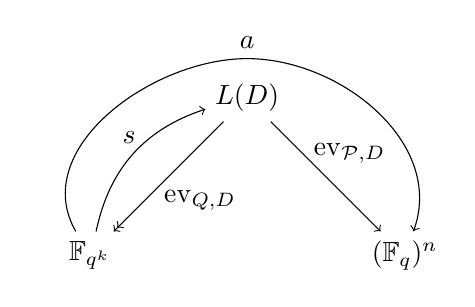
\begin{tikzpicture}
    \node (LD) at (2, 2) {$L(D)$};
    \node (Fqk) at (0, 0) {$\mathbb{F}_{q^k}$};
    \node (Fqn) at (4, 0) {$(\mathbb{F}_{q})^n$};
    \draw[->>] (LD) to (Fqk);
    \draw[->] (LD) to (Fqn);
    \draw[->] (Fqk) to[bend left] (LD);
    \node (s) at (0.5, 1.5) {$s$};
    \node (evQ) at (1.4, .7) {$\ev_{Q, D}$};
    \node (evP) at (3.3, 1.3) {$\ev_{\Pcal, D}$};
    \draw[->] (Fqk) to[out=120,in=180](2, 2.5) to[out=0, in=70] (Fqn);
    \node (a) at (2, 2.7) {$a$};
  \end{tikzpicture}
  \end{center}
  For all $1\leq i\leq n$, the map
  $x\mapsto f_x(P_i)$ is a linear form, so there exists an element
  $a_i\in\mathbb{F}_{q^k}$ such that
  \[
    \forall x\in\mathbb{F}_{q^k},\, f_x(P_i) = \ps{a_i}{x},
  \]
  thus
  \[
    \forall x\in\mathbb{F}_{q^k},\, a(x) = (\ps{a_1}{x}, \dots, \ps{a_n}{x}).
  \]
  Let $x, y, z\in\mathbb{F}_{q^k}$, and
  \[
    p = a(x)*a(y)*a(z)\in(\mathbb{F}_{q})^n
  \]
  be the coordinate-wise product of the elements $a(x)$, $a(y)$, and $a(z)$. In
  other words,
  \[
    p = (f_xf_yf_z(P_1), \dots, f_xf_yf_z(P_n)).
  \]
  Similarly, since the map $\ev_{\Pcal, 3D}$ is injective, it admits a left inverse $r$, \ie a
  map
  \[
        \begin{array}{cccc}
          r: & (\mathbb{F}_{q})^n & \to & L(D)
\end{array}
  \]
  such that
  \[
    r\circ\ev_{\Pcal, 3D} = \Id_{L(D)},
  \]
  where $\Id_{L(D)}$ is the identity map on $L(D)$. We
  also let
  \[
        \begin{array}{cccc}
          d: & (\mathbb{F}_{q})^n & \to & \mathbb{F}_{q^k} \\
\end{array}
  \]
  be the map $d = \ev_{Q, 3D}\circ r$.   The situation is sumed up in the
  following drawing.
  \begin{center}
  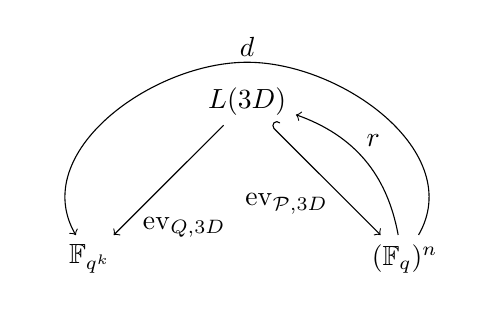
\begin{tikzpicture}
    \node (L3D) at (2, 2) {$L(3D)$};
    \node (Fqk) at (0, 0) {$\mathbb{F}_{q^k}$};
    \node (Fqn) at (4, 0) {$(\mathbb{F}_{q})^n$};
    \draw[right hook->] (L3D) to (Fqn);
    \draw[->] (L3D) to (Fqk);
    \draw[->] (Fqn) to[bend right] (L3D);
    \node (evP) at (2.5, .7) {$\ev_{\Pcal, 3D}$};
    \node (s) at (3.6, 1.5) {$r$};
    \node (evQ) at (1.2, .4) {$\ev_{Q, 3D}$};
    \draw[->] (Fqn) to[out=60,in=0](2, 2.5) to[out=180, in=120] (Fqk);
    \node (d) at (2, 2.7) {$d$};
  \end{tikzpicture}
\end{center}
The map $r$ is linear, so $d$ is also linear, by
  composition of two linear maps. Thus we have $n$ elements $d_1, \dots, d_n$ of
  $\mathbb{F}_{q^k}$ such that, for all $(x_1, \dots, x_n)\in\Img(\ev_{\Pcal,
  3D})$,
  \[
    d(x_1, \dots, x_n) = \sum_{i=1}^n x_i d_i.
  \]
Now
\[
  h = r(p)\in L(3D)
\]
is an element of $L(3D)$ such that
\[
  \forall 1\leq i\leq n,\,\ev_{\Pcal, 3D}(h) = f_xf_yf_z(P_i),
\]
but this is also the case for the function $f_xf_yf_z\in L(3D)$. Since the map
$\ev_{\Pcal, 3D}$ is injective, we have
\[
  h = f_xf_yf_z.
\]
Then, we have
\begin{equation*}
  \begin{split}
  d(p) &= \ev_{Q, 3D}(r(p))\\
  &= \ev_{Q, 3D}(h)\\
  &= h(Q)\\
  &= f_x(Q)f_y(Q)f_z(Q)\\
  &= s(x)(Q)s(y)(Q)s(z)(Q)\\
  &= \ev_{Q, D}\circ s(x)\ev_{Q, D}\circ s(y)\ev_{Q, D}\circ s(z)\\
  &= xyz.
  \end{split}
\end{equation*}
But we also have
\begin{equation*}
  \begin{split}
    p &= a(x)*a(y)*a(z)\\
    &= (\ps{a_1}{x}\ps{a_1}{y}\ps{a_1}{z}, \dots,
    \ps{a_n}{x}\ps{a_n}{y}\ps{a_n}{z}),
  \end{split}
\end{equation*}
so
\[
  d(p) = \sum_{i=1}^n\ps{a_i}{x}\ps{a_i}{y}\ps{a_i}{z}d_i
\]
and finally we have a $3$-symmetric decomposition of $m_3$:
\[
  xyz = \sum_{i=1}^n\ps{a_i}{x}\ps{a_i}{y}\ps{a_i}{z}d_i.
\]
\end{proof}
Now that we know the method to find $3$-symmetric decompositions of $m_3$, and thus
trisymmetric decompositions of $m_2$, the question is, given $q$ and $k$, to
find an algebraic function field $F/\mathbb{F}_{q}$ satisfying
Proposition~\ref{prop:method}. If $F/\mathbb{F}_q$ is a function field of genus
$g$ and $G\in\D_F$ a divisor of $F$, Riemann's theorem states that
\[
  \dim L(G) \geq \deg G + 1 - g,
\]
with equality if $\deg G > 2g - 2$. Assume that there exist $Q\in\mathbb{P}_F$ a
place of $F$ of degree $k$, $P_1, \dots, P_n$ places of degree $1$ and
$D\in\D_F$ a divisor which support does not include $Q, P_1, \dots, P_n$. Since
\[
  \Ker(\ev_{\Pcal, 3D}:L(3D)\to(\mathbb{F}_{q})^n) = L(3D-P_1-\dots-P_n),
\]
the injectivity in Condition~\eqref{cond:2} is equivalent to
\[
  L(3D-P_1-\dots-P_n)=\left\{ 0 \right\}.
\]
This is the case if
\[
\deg(3D-P_1-\dots-P_n)<0,
\]
which is the case if
\[
  n > 3\deg D.
\]
Similarly, we have
\[
  \Ker(\ev_{Q, D}:L(D)\to\mathbb{F}_{q^k}) = L(D-Q),
\]
and the rank-nullity theorem states that
\[
  \dim L(D) = \dim\Ker(\ev_{Q, D})+\dim\Img(\ev_{Q, D}),
\]
so the surjectivity in Condition~\eqref{cond:1} is equivalent to
\[
  \dim L(D-Q) = \dim L(D) - k.
\]
A sufficient condition for the last equation to hold is that
\[
  \deg D > k+ 2g - 2,
\]
because
\begin{equation*}
  \begin{split}
  \deg(D-Q) &= \deg D - \deg Q\\
  &= \deg D - k\\
  &> 2g - 2
  \end{split}
\end{equation*}
and so
\begin{equation*}
  \begin{split}
    \dim L(D-Q) &= \deg(D-Q)+1-g\\
    &=\deg D+1-g-k\\
    &=\dim L(D)-k.
  \end{split}
\end{equation*}
Thus, a sufficient condition for Conditions~\eqref{cond:1} and~\eqref{cond:2} to
hold is that
\[
  \frac{n}{3} > \deg D > k + 2g - 2.
\]
If $\frac{n}{3}>k + 2g -1$, there exists an integer $\delta\in\mathbb{N}$ with
\[
  \frac{n}{3} > \delta > k +2g -2,
\]
\eg $\delta=k+2g-1$, therefore we can assume without loss of generality that there
exists a divisor $D$ of degree $\delta$ which support does not include $Q, P_1,
\dots, P_n$, thanks to the strong approximation theorem.

The remaining part is to prove that we can find suitable function fields for
each $q$ fixed and $k\to\infty$. It means that we look for a function field
$F/\mathbb{F}_q$ of genus $g$, with a place of degree $k$, and such that there
are at least $n$ places of degree $1$, with
\[
  n > 3k +6g - 3
\]
in order to apply Proposition~\ref{prop:method}. Let us start with the special case of $q\geq64$
a square. In this case, we know~\cite{STV92} that there exists a family of function fields
$F_i/\mathbb{F}_q$ of genus $g_i$ such that
\begin{enumerate}
  \item $g_i\to\infty$
  \item $\frac{g_{i+1}}{g_i}\to1$
  \item $N_i\sim (\sqrt q - 1)g_i$
\end{enumerate}
with
\[
  N_i = \Card\left\{ P\in\mathbb{P}_{F_i}\,|\,\deg P = 1 \right\}
\]
the number of places of degree $1$ of $F_i$. We also assume that the sequence
$(g_i)_i$ is increasing. For each $k$, let $g_{i(k)}$ be the
smallest genus $g_i$ such that
\[
  N_{i} > 3k + 6g_{i}.
\]
This is always possible to find such an index $i(k)$ since
\[
  N_i\sim (\sqrt q - 1)g_i
\]
and $\sqrt q -1 > 6$. By definition, we thus have
\[
  N_{i(k)-1}\leq 3k+6g_{i(k)-1}<3k+6g_{i(k)}<N_{i(k)}.
\]
Since $i(k)\to\infty$ when $k\to\infty$, we can use the asymptotic results on the
family of function fields $F_i$, so we know
\begin{equation*}
  \begin{split}
  N_{i(k)-1} &\sim (\sqrt q-1)g_{i(k)-1}\\
  &\sim (\sqrt q-1)g_{i(k)}\\
  &= (\sqrt q-1)g_{i(k)}+o(g_{i(k)}).
  \end{split}
\end{equation*}
Similarly,
\[
  N_{i(k)} = (\sqrt q -1)g_{i(k)}+o(g_{i(k)}),
\]
and so we deduce that
\begin{equation}
  3k = (\sqrt q -7)g_{i(k)} + o(g_{i(k)})
  \label{eqn:equivg}
\end{equation}
and
\begin{equation}
  g_{i(k)}= \frac{3}{\sqrt q - 7}k+o(k).
  \label{equivk}
\end{equation}
We know~\cite[Corollary 5.2.10.]{Stichtenoth09} there exists a place of degree
$k$ in $F_{i(k)}$ if we have
\begin{equation}
  2g_{i(k)} +1 \leq q^{(k-1)/2}(\sqrt q-1),
  \label{eqn:degreek}
\end{equation}
but thanks to Equation~\eqref{eqn:equivg} we know that
Inequation~\eqref{eqn:degreek} is true as soon as $k$ is large enough. Let
$k_0(q)$ be a constant such that~\eqref{eqn:degreek} is true for $k\geq k_0(q)$.
If $q\geq 64$ is a square and $k\geq k_0(q)$, we now know that we can find a
function field $F_{i(k)}$ in which Proposition~\ref{prop:method}
applies, so that we can find a $3$-symmetric decomposition of $m_3$ of length
$n$, and therefore a trisymmetric decomposition $\mathbb{F}_{q^k}/\mathbb{F}_q$ of length $n$, with
\begin{equation*}
  \begin{split}
    n&\leq N_{i(k)}\\
    &= (\sqrt q -1)g_{i(k)}+o(g_{i(k)})\\
    &= \frac{\sqrt q -1}{\sqrt q -7}\cdot3\cdot k+o(k)\\
    &= O(k).
  \end{split}
\end{equation*}
We have thus proven that the trisymmetric bilinear complexity of
$\mathbb{F}_{q^k}/F_{q}$ is \emph{linear} in $k$ for $q\geq64$ a square.

Let $q\geq3$ be a prime power, there exists an integer $d\in\mathbb{N}$ such that
\[
  q' = q^d \geq 64
\]
is a square. Let $\sym{q}{k}$ be the minimal length of a $3$-symmetric
decomposition of
\[
  m_3:\mathbb{F}_{q^{k}}\times\mathbb{F}_{q^k}\times\mathbb{F}_{q^k}\to\mathbb{F}_{q^k}.
\]
We know that there exists some constant
$N$ such that
\[
  \sym{q'}{k}\leq Nk
\]
for $k$ large enough, and since we know that

\[
  \sym{q}{kd}\leq\sym{q'}{k}\sym{q}{d},
\]
it follows that
\[
  \sym{q}{kd} \leq (sN)k.
\]
\begin{center}
  \begin{tikzpicture}
    \node (Fq) at (0, 0) {$\mathbb{F}_q$};
    \node (Fqk) at (-2, 2) {$\mathbb{F}_{q^k}$};
    \node (Fqd) at (2, 2) {$\mathbb{F}_{q'}$};
    \node (Fqkd) at (0, 4) {$\mathbb{F}_{q'^{k}}$};
    \draw (Fq) -- (Fqd);
    \draw (Fqd) -- (Fqkd);
    \draw (Fqk) -- (Fqkd);
    \draw (Fq) -- (Fqk);
    \node (s) at (1.2, .9) {$s$};
    \node (Ok) at (1.5, 3.1) {$N$};
  \end{tikzpicture}
\end{center}
Since
\[
  \mathbb{F}_{q^k}\subset\mathbb{F}_{q'^k}\cong\mathbb{F}_{q^{kd}},
\]
we also have
\begin{equation*}
  \begin{split}
    \sym{q}{k}&\leq\sym{q}{kd}\\
    &\leq (sN)k.
  \end{split}
\end{equation*}
Because $\tri{q}{k}\leq\sym{q}{k}$, it thus proves that the trisymmetric bilinear complexity of
$\mathbb{F}_{q^k}/\mathbb{F}_q$ is asymptotically linear in $k$, for any $q\geq3$.

\bibliographystyle{plain}
\bibliography{erou}

\end{document}
